\begin{enumerate}
	\item l'utilisateur choisit la session correspondante à sa demande.
	\item l'utilisateur click sur le bouton +
	\item Si le bouton + n'est pas grisée l'utilisateur peut s'inscrire et possède donc encore des sessions dans son abonnement
\end{enumerate}

\vspace{\baselineskip}
\begin{figure}[h]
	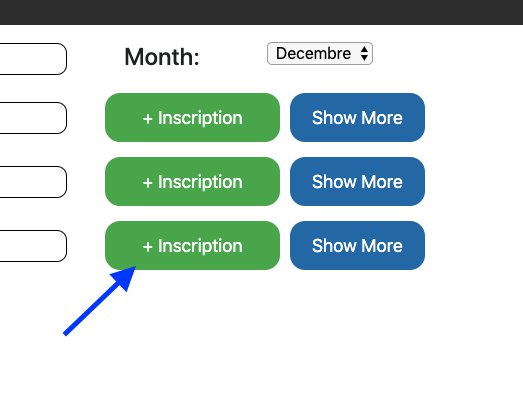
\includegraphics[width=0.5\textwidth,center]{Figures/us3-1}
	\caption{Bouton d'inscription quand abonnement rempli}
\end{figure}

\newpage
\begin{figure}[h]
	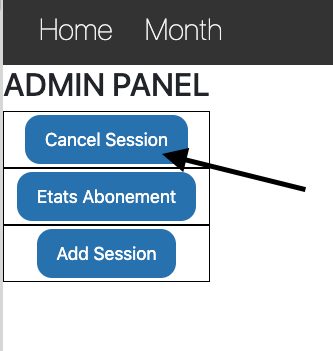
\includegraphics[width=0.4\textwidth,center]{Figures/us9-1}
	\caption{Bouton d'inscription quand abonnement vide}
\end{figure}
